% =====================================================================================
% DEDV_2.tex -- FAITHFUL TRANSCRIPTION of "DEDV (2).pdf" (report/DEDV_2_original.pdf).
%
% No .tex source of the paper existed, so this file was rebuilt from the PDF: same text,
% same errors, same structure. Hyphenation at line ends was joined. Figures 1-2 are
% redrawn in TikZ and Fig. 3 is drawn from the counts printed in the PDF.
%
% Where the PDF shows a sentence cut off after a number (Sec. 7 "...with 72.5", Sec. 7.1
% "...close to 15.9"), the cause is an unescaped "%" in the original source: everything after
% it on that line became a comment. The lost text is unknown, so this file reproduces the cut.
%
% Do not edit this file. All corrections are in DEDV_2_revised.tex (see REPORT_CHANGES.md).
% Build: pdflatex DEDV_2 && bibtex DEDV_2 && pdflatex DEDV_2 && pdflatex DEDV_2
% =====================================================================================
\documentclass[pdflatex,sn-mathphys-num]{sn-jnl}

\usepackage{graphicx}%
\usepackage{multirow}%
\usepackage{amsmath,amssymb,amsfonts}%
\usepackage{xcolor}%
\usepackage{textcomp}%
\usepackage{booktabs}%
\usepackage{tikz}%
\usetikzlibrary{positioning,arrows.meta}%
\usepackage{pgfplots}%
\pgfplotsset{compat=1.18}%
\usepgfplotslibrary{colorbrewer}%

\raggedbottom

\begin{document}

\title[DEDV]{DEDV - A Dynamic Encryption Digital Vault for a secured document storage}

\author[1]{\fnm{K.T.} \sur{Hiranmayi}}\email{hiranmayi.23bcb7022@vitapstudent.ac.in}
\author*[1]{\fnm{Ngangbam} \sur{Indrason}}\email{indrason.n@vitap.ac.in}
\author[1]{\sur{Soumya}}\email{soumya.23bcb7020@vitapstudent.ac.in}
\author[1]{\sur{Swapnil}}\email{swapnil.23bcb7031@vitapstudent.ac.in}
\author[1]{\fnm{Pallam} \sur{Sneitha}}\email{snehita.23bcb7237@vitapstudent.ac.in}

\affil*[1]{\orgdiv{School of Computer Science and Engineering}, \orgname{VIT-AP University},
\orgaddress{\city{Amaravati}, \postcode{522241}, \state{Andhra Pradesh}, \country{India}}}

\abstract{Different Security requirements of individual documents may not be accounted for by
conventional document storage. This paper presents Dynamic Encryption Digital Vault (DEDV), a
unified document storage framework that uses context and document related attributes to predict
security level and configure encryption. Five machine learning models K Nearest Neighbors (KNN),
Decision Tree (DT), XGBoost (XGB), Multinomial Logistic Regression (MLR) and Random Forest (RF)
were evaluated using experimental survey data comprising 402 records from 67 responses. Random
Forest achieved a macro F1 score of 0.398$\pm$0.026 using ten input features. A reduced seven
input configuration achieved 0.380$\pm$0.024 and was selected based on predefined criteria
balancing input reduction, classification performance and under classification risk. The system
combines a security level prediction with vault specific encryption configurations and token based
key management framework. Enhanced class contains only eight records, resulting in limited
classification reliability. Further research should expand the dataset, validate the model using
more representative data and evaluate the system with real world documents.}

\keywords{Dynamic encryption, Digital vault, Security level classification, Random Forest, Key
management}

\maketitle

\section{Introduction}\label{sec1}

Cloud platforms and digital libraries are preferred for data storage instead of storing the data
exclusively locally \cite{asim2026adoption}. This makes it easy to use and access the data but
also creates the concern of security and protection of the data.

Encrypting each file with the highest security seems good but results in more storage and time
consumption. Thus the required protection for data or a document depends on various factors
including circumstances in which it will be used. A document containing normal data may not
require the same level of protection as one containing confidential business information or a
document containing personal information. Using the same protection method for all the data being
stored won't account for these differences. The level of protection a document needs will depend
on various factors including document sensitivity, file type, content classification, ownership,
user role, sharing requirements, access frequency, and the risk associated with unauthorized
access \cite{khan2023cybersecure}\cite{smallwood2012safeguarding}\cite{phoha2014context}. Access
requirements from multiple devices and retention can also affect the level of protection required
for the document. Hence, considering the context of usage and features of the document must be
considered while implementing protection protocols.

Encryption is necessary while protecting the data and the choosing the type of encryption
algorithm is a part of implementing the security \cite{akinkunmi2024importance}. The storage
system must also maintain the encryption along with keys and user access to the data in the
storage. When authorized user is accessing the data It is necessary to retrieve the decryption key
for user access. These operations should work together for consistent document protection during
storage and retrieval.

Previous papers delt with cloud storage, data classification, Machine learning models and
encryption algorithms for secure data storage in digital and cloud models. The Confidentiality
based Data Classification-as-a-Service(C2aas) approach emphasis on how data can be classified
based on confidentiality requirements and how the classification can help with the encryption
decision in cloud environments. The idea of classification of level of protection based on the
confidentiality requirement of the data rather than using the same level of security for every
item \cite{ali2023confidentiality}. Jabbar and Bhaya proposed a private cloud security approach
that deals with machine learning, data classification and cryptographic methods. Network attack
deatection along with user data classification based on importances and application of different
encryption algorithm is considered in their work \cite{jabbar2022secure}. This provides a related
example for machine learning model to support security required and differentiate data
protection. Another model deals with the classification of cloud data to enhance security by
adding data characteristics and security requirements with selecting the type of encryption
required \cite{singh2018classification}. The border relevance with this work is classification can
provide basis for implementing appropriate protection mechanism based on requirements of the data
being stored. Machine learning has also been delt with cloud encryption and retrieval. Malhotra
and Singh researched on key-word ranking approach using artificial neural network based on
data-encrypiton. Their work considers the usage of Machine learning in encryption and retrieval
rather than just using it for general data classification \cite{malhotra2023efficacy}.
Confidential Machine Learning deals with another aspect of this problem. Machine learning and
protecting sensitive information protection may not be fully trusted while using in these
platforms. Techniques delt with in this approach include homomorphic encryption, hybrid
cryptographic protocols, garbled circuits, perturbation-based methods and hardware assisted
approaches. These techniques have a trade-off between confidentiality, computational cost and
model utility \cite{sagar2021confidential}. Together these studies provide different backgrounds
for various components. Their approaches are different and they focus on different security
objective.

The reviewed studies establish that data classification, machine learning, encryption, and
cryptographic protection have already been explored in cloud-security research
\cite{thabit2023data}. The research gap here should therefore not be framed as the absence of
machine learning or encryption in existing systems. Instead, the gap concerns the particular
combination being investigated. We consider document characteristics alongside user and
usage-context parameters when predicting the required security level. It defines separate personal
and enterprise security hierarchies, evaluates candidate machine-learning models for the
prediction task, and links the resulting classification to an encryption configuration. The
framework also incorporates tokenized key management into the document-protection workflow. The
token provides a reference for locating the key associated with an encrypted document during an
authorized retrieval operation. This brings security-level assignment, encryption configuration
selection, and key association into one proposed digital-vault design. The contribution should be
described in terms of this integration and its evaluation. It should not imply that the
individual machine-learning models, encryption techniques, or token-based references are new
inventions.

The Dynamic Encryption Digital Vault (DEDV) is designed as a framework for document storage that
connects the level of security required based on the prediction from a Machine learning model and
encrypting the document. For user access a controlled document retrieval system is implemented.
The main idea is to determine the required level of protection for a documents based on available
parameters of the document and contextual data\cite{sasikumar2025enhancing}.

The main contributions of the proposed work can be presented as follows:
\begin{itemize}
\item DEDV deals with all the following mentioned points.
\item Context-based security-level prediction: The framework uses document-related and contextual
parameters to determine the security level assigned to a document.
\item Separate personal and enterprise hierarchies: DEDV provides two environments for document
storage including personal vault with three levels of security and Enterprise vault with five
levels of security.
\item Comparative evaluation of machine learning models: Five models - KNN, RF, XGB, MLR, and DT
are evaluated for security level prediction with final model being Rf after using experimental
results.
\item Security level to encryption mapping: The predicted level is mapped to the associated
encryption algorithm.
\item Tokenized key-management workflow: The framework separates encryption keys from encrypted
documents and uses tokenized references to support key retrieval during authorized decryption.
\end{itemize}

DEDV addresses how a document attributes and usage context information can be considered while
assigning a security level and mapping an encryption and key management

DEDV proposes two security hierarchies. The personal vault consists of three security levels and
the enterprise vault consists of five security level with an option to choose between two
encryptions for the final security level. The system uses a mapping between each security level
and its corresponding encryption algorithm. This framework allows two different environments
within a single secure vault.

During the decision process various parameters as document sensitivity, file type, file size,
content classification, user role, organization type, ownership, access frequency, sharing
requirements, risk level, multiple-device access and retention period are considered. These
characteristics of a document cover various accepts of the document and their intended use. The
level of protection required is determined by the relevant information provided to the
classification model.

Five Machine learning models are considered for the prediction task: K-Nearest Neighbors (KNN),
Random Forest (RF), XGBoost (XGB), Multinomial Logistic Regression (MLR), and Decision Tree (DT).
These models are compared using experimental data sets and the final decision engine Is
determined by observed evaluation results.

DEDV also proposes encryption key separation and tokenized key management. The encryption key is
stored separately and a token serves as a reference to associated decryption key. When a document
is retrieved, the system first checks for authorization before retrieving the decryption key. The
token serves as a reference to the encryption key. It supports the mapping and the retrieval
process.

DEDV connects four related operations: Determining the security level , selecting the mapped
encryption algorithm, managing the encryption key and control the retrieval process.

This paper is organized as follows. Section 2 discussed about the various related works. The
motivation of this work is laid down in Section 3. The proposed system model is discussed in
detail in Section 4. Section 5 describes the working methodology of the proposed system. The
experimentation is shown in Section 6. The results and discussion of the experimentation are given
in Section 7. Section 8 deals with the limitation of the proposed work. The future scope of work
is discussed in Section 9 and Section 10 concludes the paper.

\section{Related Works}\label{sec2}

Research on protected digital storage has explored machine learning, data classification,
cloud-based encryption and cryptographic techniques. The aim of these studies is to protect data
while considering factors like confidentiality, computational overhead and the efficiency of data
storage and retrieval. The following works are relevant to the development of the Dynamic
Encryption Digital Vault (DEDV).

\subsection{Confidentiality-Based Data Classification-as-a-Service (C2aaS)}

Ali et al. \cite{ali2023confidentiality} proposed Confidentiality-based Data
Classification-as-a-Service (C2aaS) to address the security and processing overhead associated
with cloud data storage. The authors of this paper focus on confidentiality risks created by
storing data in plaintext and how encrypting the data can increase processing requirements. Their
proposed model classifies data according to security level and before clous storage it is
processed dynamically. The objective is to secure confidential data while reducing unnecessary
system overhead. C2aaS is closely related to DEDV because both approaches use security
classification to determine how data should be handled. However, DEDV focuses on a digital-vault
framework in which document characteristics and usage-context parameters contribute to a
predicted security level. It also defines separate security hierarchies for personal and
enterprise environments and connects the predicted level to an encryption configuration and
tokenized key-management workflow.

\subsection{Security of Private Cloud using ML and Cryptography}

Jabbar and Bhaya proposed a security model for private cloud environments that combines network
attack detection with data classification and encryption. Their approach has two phases. In the
first phase normal and abnormal traffic is detected whereas the second classifies the user data
according to its importance and applies different encryption algorithm. The authors evaluate
machine learning algorithms for attack detection and data classification, including Random
Forest, Decision Tree, Logistic Regression, and Stochastic Gradient Descent
\cite{jabbar2022secure}. This work demonstrates how machine learning can support different
security operations in a cloud environment. Its approach is relevant to DEDV because it links data
classification with the selection of encryption methods. DEDV focuses on predicting the required
security level of an individual document using a comparison of five models. The selected model is
then used as the decision engine within the vault's personal or enterprise security hierarchy.

\subsection{Classification of Data to Enhance Data Security in Cloud Computing}

The study Classification of Data to Enhance Data Security in Cloud Computing examines how data
classification can support the selection of suitable encryption methods in cloud environments.
The authors explain that data security requirements vary according to the type of information and
the requirements of its owner. Their work proposes classifying cloud data using relevant security
parameters so that an appropriate encryption method can be selected dynamically
\cite{singh2018classification}. This study supports the principle that different data items may
require different levels of protection. It focuses on the relationship between encryption and
classification efficiency. DEDV builds on this general principle by considering a combination of
document, user, and usage-context parameters in its security-level decision process. It also
distinguishes personal and enterprise storage requirement rather than a single hierarchy for both
environments.

\subsection{An Efficacy Analysis of Data Encryption Architecture for Cloud Platform}

The authors of An Efficacy Analysis of Data Encryption Architecture for Cloud Platform propose a
machine-learning-based model for cloud data encryption and retrieval. This model combines
Symmetric Searchable Encryption with a keyword ranking method based on Artificial Neural Network
(ANN). The study compares the proposed model with multiclass Support Vector Machine (SVM) and
Na\"{\i}ve Bayes approaches and evaluates its operational performance using measures that include
the true-positive rate and false-positive rate \cite{malhotra2023efficacy}. This work is relevant
because it applies machine learning within a cloud encryption and retrieval architecture. It shows
that machine learning can contribute to security-related operations beyond conventional data
classification. DEDV focuses on predicting a document's required security level and uses that
prediction to the mapped encryption algorithm. The five candidate models in DEDV are evaluated for
this security-level prediction task.

\subsection{Confidential Machine Learning on Untrusted Platforms: A Survey}

Sagar and Chen presented a survey of confidential machine learning on untrusted platforms,
including public cloud and edge environments. This study focuses on machine learning and
cryptographic approaches for protecting sensitive training data during outsourced computation.
This study focuses on hybrid cryptographic protocols, homomorphic encryption, garbled circuits,
perturbation-based method and hardware assisted approaches. The authors examined the trade off
between model utility, confidentiality and computational cost
\cite{asikis2020optimization}\cite{sagar2021confidential}. This survey provides a broader security
perspective for systems that combine machine learning with outsourced
computing\cite{jauernig2020trusted}. It is relevant to DEDV because a secure vault must consider
not only how a document is encrypted but also how sensitive information and associated operations
are protected. The survey focuses on confidentiality machine learning rather than a vault for
documents that predicts security levels, and then maps them to encryption configurations and
manages document access through tokenized key references.

\subsection{Comparative Analysis of Existing Work}

Table~\ref{tab1} presents a comparison of the reviewed studies, highlighting their main focus,
relevant contributions, and relationship to the proposed DEDV system.

The reviewed studies establish that data classification, machine learning, encryption, and
cryptographic protection have already been explored in cloud-security research. Therefore, the
motivation for DEDV is not simply to combine machine learning with encryption, since previous
work has already investigated related combinations.

The reviewed studies address different aspects of cloud security, data classification,
encryption, and machine learning. Their main contributions and their relationship to DEDV are
summarized below.

\begin{table}[h]
\caption{Comparison of Existing Studies with the Proposed DEDV}\label{tab1}
\begin{tabular}{@{}cp{3cm}p{3.6cm}p{3.6cm}@{}}
\toprule
Reference & Main Focus & Relevant Contribution & Relationship to DEDV \\
\midrule
\cite{ali2023confidentiality} & Confidentiality-based data classification for cloud storage &
  Dynamically handles data according to its security level & Supports security-level-based data
  handling \\
\cite{jabbar2022secure} & Private-cloud security using machine learning and cryptography &
  Combines attack detection, data classification, and encryption & Demonstrates ML-based
  classification linked to encryption \\
\cite{singh2018classification} & Data classification for cloud security & Uses data
  classification to guide encryption selection & Supports differentiated protection based on
  data requirements \\
\cite{malhotra2023efficacy} & Machine-learning-based cloud encryption and retrieval & Combines
  searchable encryption with ANN-based keyword ranking & Demonstrates ML integration within an
  encryption and retrieval architecture \\
\cite{sagar2021confidential} & Confidential machine learning on untrusted platforms & Surveys
  cryptographic and other techniques for protecting ML computations & Provides background on
  confidentiality and cryptographic protection \\
\botrule
\end{tabular}
\end{table}

\subsection{Research Gap}

Instead, the proposed work focuses on integrating these capabilities within a single
digital-vault framework. DEDV considers document characteristics together with user and
usage-context parameters to predict the required security level. It defines three levels for the
personal vault and five levels for the enterprise vault, evaluates five candidate machine learning
models for the prediction task, and uses the selected model to determine the corresponding
encryption configuration. The framework also includes a tokenized key management to support
controlled key association and retrieval during authorized decryption.

Based on the five studies reviewed here, this particular combination of context-based
security-level prediction, separate personal and enterprise hierarchies, encryption-configuration
selection, and tokenized key management provides the direction for DEDV. The contribution lies in
the integration and evaluation of these components, rather than in claiming that each component is
individually new.

\section{Motivation}\label{sec3}

\subsection{Motivation}

Existing works have explored machine learning, classification and encryption to improve security
of the data. The protection required depends on factors other than its content such as
sensitivity, exposure consequences, access reequipments and duration of protection required will
also affect the security level needed. DEDV focuses these factors while assigning the security
levels to stored document.

The proposed model also considers contextual parameters to predict the security level required
for the document. Personal vault environment has three security levels and Enterprise vault has
five levels of security with an option to choose among two encryption algorithms in the final
level. This structure allows the structure to predict the protection level according to the
required environment rather than using the same hierarchy for every document.

DEDV is tested using five Machine learning models: K-Nearest Neighbors (KNN), Random Forest (RF),
XGBoost (XGB), Multinomial Logistic Regression (MLR), and Decision Tree (DT). Random Forest is used
as decision engine based on model selection process \cite{speiser2019comparison}. Random Forest is
used as a decision engine. Its purpose is to take input parameters and choose appropriate security
level and map it the corresponding encryption configuration.

Tokenized key management is also incorporated in the framework. Encryption documenta and
encryption keys are stored separately and tokens provide a reference to the associated decryption
keys. During document retrieval, authorization is confirmed before decryption. This forms the
connection between security level prediction with encryption and controlled document access.

\subsection{Challenges}

Parameters selecting is one of the challenges in DEDV that provide useful information for security
level prediction. Random Forest model uses seven input parameters: Sensitivity, Who Should Access,
Access Frequency, Exposure Consequence, Protection Duration, Multiple Locations and Multiple
Devices. These inputs consider different aspects of document sensitivity and the context of usage
and their representation should remain same between prediction and training.

Mapping the predicted security to the corresponding encryption configuration is another
configuration. The system considers the vault type before configuration as personal and enterprise
vaults have different security levels within the environment. An incorrect mapping might result in
unnecessary encryption that does not map with the assigned level.

The encryption key and encrypted document are separately maintained; key management introduces
another challenge. The system must preserve the association between the document, its token and
corresponding key. During decryption and retrieval, authorization must be verified before the key
is released. To maintain the intended document protection work flow it is necessary to maintain
the association and restricting key access.

\section{Proposed System Model}\label{sec4}

Fig.~\ref{fig1} is the illustrated proposed system model of Dynamic Encryption Digital Vault
(DEDV). The Security level required is predicted by contextual and document related parameters.
Machine learning model used for decision making is Random Forest, it takes seven inputs and
classifies the document into one of four security levels: Low, Standard, Enhanced and
High/Critical\cite{phoha2014context} Figure~\ref{fig1} illustrates the DEDV workflow, from
contextual security-level prediction to vault-specific encryption configuration, separate key
management, and authorized document retrieval.

The vault Environment also plays part in the predicted security level. The Enterprise vault
contains five security levels and the personal vault contains three security levels. The system
maps corresponding encryption to the respective security level of relevant vault
environment\cite{sasikumar2025enhancing}. The System predicts security level and does not directly
assign the encryption algorithm.

\begin{figure}[h]
\centering
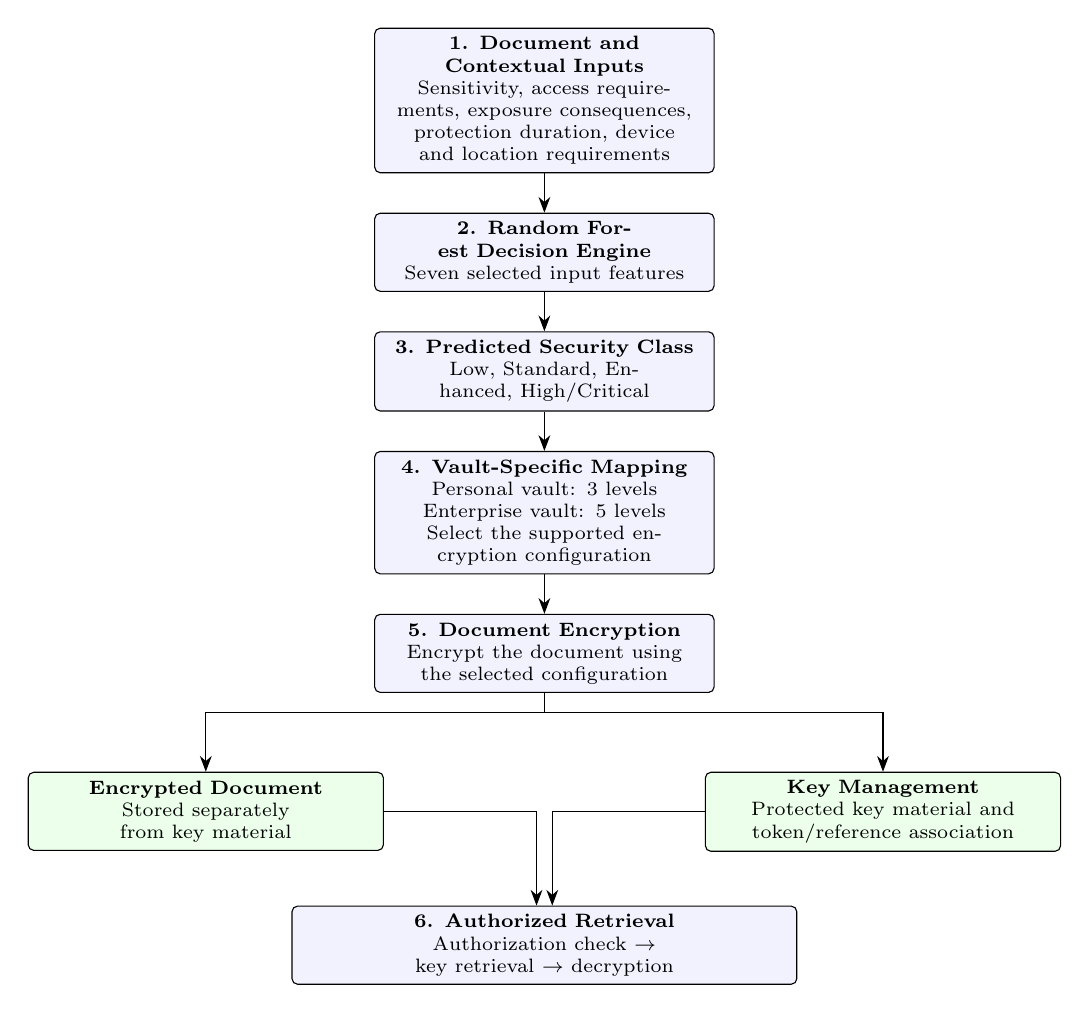
\begin{tikzpicture}[
  box/.style={draw, fill=blue!5, rounded corners=2pt, align=center, text width=4.1cm,
              font=\scriptsize, inner sep=3pt},
  side/.style={draw, fill=green!8, rounded corners=2pt, align=center, text width=4.3cm,
               font=\scriptsize, inner sep=3pt},
  arr/.style={-{Stealth[length=2mm]}},
  node distance=5mm]
\node[box] (b1) {\textbf{1. Document and Contextual Inputs}\\ Sensitivity, access requirements,
  exposure consequences, protection duration, device and location requirements};
\node[box, below=of b1] (b2) {\textbf{2. Random Forest Decision Engine}\\ Seven selected input
  features};
\node[box, below=of b2] (b3) {\textbf{3. Predicted Security Class}\\ Low, Standard, Enhanced,
  High/Critical};
\node[box, below=of b3] (b4) {\textbf{4. Vault-Specific Mapping}\\ Personal vault: 3 levels\\
  Enterprise vault: 5 levels\\ Select the supported encryption configuration};
\node[box, below=of b4] (b5) {\textbf{5. Document Encryption}\\ Encrypt the document using the
  selected configuration};
\node[side, below=10mm of b5, xshift=-4.3cm] (enc) {\textbf{Encrypted Document}\\ Stored
  separately\\ from key material};
\node[side, below=10mm of b5, xshift=4.3cm] (km) {\textbf{Key Management}\\ Protected key
  material and\\ token/reference association};
\node[box, below=27mm of b5, text width=6.2cm] (b6) {\textbf{6. Authorized Retrieval}\\
  Authorization check $\rightarrow$ key retrieval $\rightarrow$ decryption};
\foreach \a/\b in {b1/b2, b2/b3, b3/b4, b4/b5}
  \draw[arr] (\a) -- (\b);
\draw (b5.south) -- ++(0,-2.5mm) coordinate (split);
\draw[arr] (split) -| (enc.north);
\draw[arr] (split) -| (km.north);
\draw[arr] (enc.east) -| ([xshift=-1mm]b6.north);
\draw[arr] (km.west) -| ([xshift=1mm]b6.north);
\end{tikzpicture}
\caption{Proposed architecture of the Dynamic Encryption Digital Vault (DEDV).}\label{fig1}
\end{figure}

Once encryption algorithm is selected, the document is encrypted and stored separately from the
key. A token provides reference to the associated key. This provides independent key retrieval
from document storage.

When a document is requested, the authorization is verified by the system before retrieving the
associated key. Once access is granted, the key is used for decrypting the document. Unauthorized
requests will not get any the key.

The proposed DEDV hence connects secure document storage and retrieval with security level
prediction, encryption configuration mapping, key management within a single unified vault
environment. Classification is performed by Random Forest and subsequent components hondle
authorized access and document protection.

\section{Methodology}\label{sec5}

In DEDV the methodology includes selecting the parameters, preparing the dataset, comparing
machine learning models, and using the predicted security level to select the encryption
configuration. Information about the document and its usage is considered by the system to
determine the protection required. Security prediction is determined by selected level, then
encryption and key management are carried out

\subsection{Selection of Parameters}

The first step in DEDV is to identify the parameters that can influence the security requirement
of a document. The system considers both document characteristics and the context in which the
document is used. Document-related parameters include sensitivity, file type, file size, and
content classification. User role, organization type, ownership, access frequency, sharing
requirement, risk level, multiple-device access, retention period are contextual
parameters\cite{phoha2014context}.

The level of protection required may vary depending on the document and its intended use hence
these parameters are considered. For example, a normal document will require less protection than
a document containing sensitive information . The access and sharing requirements can affect how
the document should be protected. With these factors in consideration, the security level decision
is made using more than one attribute.

The selected parameters are provided as inputs to the machine learning models. They need to be
represented in a format suitable for processing, depending on the type of data. The parameters
available in the experimental dataset are used for the prediction task. Their influence on the
final prediction is also important, as different parameters may contribute differently to the
security-level decision.

\subsection{Evaluation of Machine Learning Models}

Five machine Learning models were tested for the security level prediction: K-Nearest Neighbours
(KNN), Random Forest (RF), XGBoost (XGB), Multinomial Logistic Regression (MLR) and Decision Tree
(DT). Classification is approached differently in each Machine Learning
Model\cite{theng2024feature}. In KNN prediction is made by considering nearby data points, whereas
in Decision Tree, a few conditions are followed. Multiple decision trees are used in Random Forest
and In Multinomial Logistic Regression, classification across several classes is handled. A new
tree is built in sequence with each tree helping the new one in the XGBoost Machine Learning model.
The experimental data set is used to compare the models. From the results, The better performing
model among all is Random Forest, Hence it is chosen for the final Framework. Other models
provided a basis of comparison for the prediction model.

\begin{figure}[h]
\centering
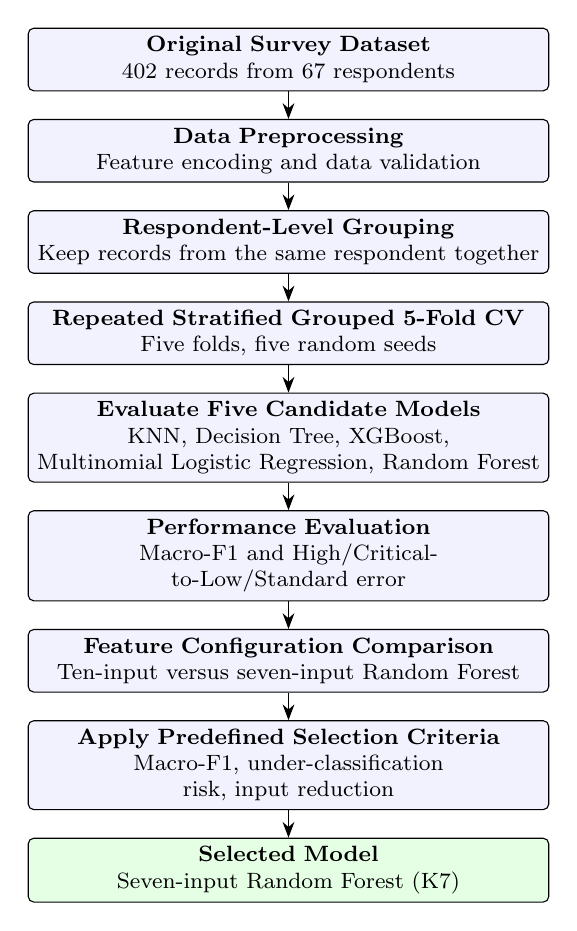
\begin{tikzpicture}[
  stp/.style={draw, fill=blue!5, rounded corners=2pt, align=center, text width=6.4cm, font=\footnotesize,
               inner sep=3pt},
  arr/.style={-{Stealth[length=2mm]}},
  node distance=3.5mm]
\node[stp] (s1) {\textbf{Original Survey Dataset}\\ 402 records from 67 respondents};
\node[stp, below=of s1] (s2) {\textbf{Data Preprocessing}\\ Feature encoding and data validation};
\node[stp, below=of s2] (s3) {\textbf{Respondent-Level Grouping}\\ Keep records from the same
  respondent together};
\node[stp, below=of s3] (s4) {\textbf{Repeated Stratified Grouped 5-Fold CV}\\ Five folds, five
  random seeds};
\node[stp, below=of s4] (s5) {\textbf{Evaluate Five Candidate Models}\\ KNN, Decision Tree,
  XGBoost,\\ Multinomial Logistic Regression, Random Forest};
\node[stp, below=of s5] (s6) {\textbf{Performance Evaluation}\\ Macro-F1 and High/Critical-\\
  to-Low/Standard error};
\node[stp, below=of s6] (s7) {\textbf{Feature Configuration Comparison}\\ Ten-input versus
  seven-input Random Forest};
\node[stp, below=of s7] (s8) {\textbf{Apply Predefined Selection Criteria}\\ Macro-F1,
  under-classification\\ risk, input reduction};
\node[stp, below=of s8, fill=green!10] (s9) {\textbf{Selected Model}\\ Seven-input Random Forest (K7)};
\foreach \a/\b in {s1/s2, s2/s3, s3/s4, s4/s5, s5/s6, s6/s7, s7/s8, s8/s9}
  \draw[arr] (\a) -- (\b);
\end{tikzpicture}
\caption{Experimental methodology for model evaluation and feature selection.}\label{fig2}
\end{figure}

Figure~\ref{fig2} Provides how the final Random Forest method is selected from experimental
procedures, including model evaluation, respondent level grouping, feature comparison and
selection.

\subsection{Prediction of Security Level}

The security level required for each document is predicted by the selected Random Forest Machine
Learning model. The document parameters and the context in which it is used will decide the
prediction. The security level is then decided by the results and it will decide the encryption
assignment.

The type of vault is also necessary in the decision making process.The personal vault has three
levels of security and the enterprise vault has five levels of security. The two vaults have
different levels of hierarchy and the framework identifies the required prediction level.Then,
based on the assigned level, the encryption level is decided. The selected configuration must
correspond with the assigned level to the document. This output from the model and the actual
protection is applied to the system.

\subsection{Selection of Encryption Configuration}

The security level assigned to the document is based on the selected encryption
configuration\cite{sasikumar2025enhancing}. The same mapping cannot be used for both personal and
enterprise vault because the personal and enterprise vault use their own hierarchy levels. A
mapping between the security levels and their encryption configuration is maintained. To identify
the correct security level configuration, the framework uses both personal and enterprise vaults.
If the mapping is not correct it could lead to improper encryption assignment. During retrieval,
token is used to associate the key. In retrieval , the key is kept separate from the file to
ensure security. The framework must maintain a proper key linkage to the requested document and it
is released only when the access is authorized.

\subsection{Tokenized Key Management}

The encrypted document and the encryption key are kept apart in DEDV. A token refers to the key
that is connected to a document\cite{rana2023comprehensive}.It assists the system in determining
which key is needed for decryption rather than containing the key itself. The relationship between
the document, its token, and the related key must be maintained by the system.Without this
association, it becomes challenging to retrieve the relevant key, and the document might not be
correctly decrypted. The token is used to locate the related key when a document has to be
accessed.Key retrieval is a discrete step in the process since the key is kept apart from the
file.The system must still make sure that the requested document is linked to the proper key and
that it is only released when access is authorised.

\subsection{Document Retrieval and Decryption}

Upon document request, the framework checks if the request is authorized.Upon successful
authorization, permission is granted. If permission is granted then the token is used to find out
the corresponding encryption key. If authorization is not successful the encryption key will not
be released. For retrieval process access control along with decryption should be performed for
every request. The Required security level is determined by the model, then the mapped
configuration is applied and the tokenized key management helps with access to the encrypted
document when there is a request

\section{Experimentation}\label{sec6}

The experimentation was carried out to evaluate the machine learning models used for
security-level prediction in DEDV. The main aim was to compare the five models and identify which
one gives the best result for the classification task. The experiments also consider how the
predicted security level is connected to the encryption process in the personal and enterprise
vaults.

\subsection{Experimental Setup}

Five Machine Learning models are used for experiments including K-Nearest Neighbors (KNN), Rando
Forest (RF), XGBoost (XGB), Multinomial Logistic Regression (MLR) and Decision Tree (DT). To compare
the performance, five models are evaluated for the same prediction task.Random Forest is selected
for the final decision engine based on the results obtained during experimentation.

The dataset contains document-related and contextual parameters used to determine the required
security level. These parameters provide the information needed by the models to make their
predictions. The experimental setup focuses on classification performance and the use of the
predicted level in the DEDV workflow.

\subsection{Comparison of Machine Learning Models}

To predict the security level suitable for the document, five models were
compared\cite{theng2024feature}. Each Machine Learning model uses its own method to classify the
input data and the results provided a basis for comparison and selecting the final model. The best
results were achieved by the Random Forest model (RF) among the evaluated models used to select the
security level for DEDV. The other four models are used for comparison and selecting the final
model for DEDV.

\subsection{Security-Level Assignment}

After comparison and selection of Random Forest for Security level prediction, characteristics of
the document and contextual parameters are used as inputs for the prediction. Then the output is
used to map the encryption algorithm for predicted security level. The vault environment is also
considered for the security level assignment. The personal vault has three security levels and the
enterprise level has five security levels. During the security prediction, the vault environment
is also taken into consideration. This part focuses on the connection between the encryption and
output stages. The selected security level corresponds to the mapped encryption algorithm.

\subsection{Encryption and Key Management}

The next part of the experimentation concerns the use of the selected encryption configuration and
the handling of encryption keys. Once a security level has been assigned, the corresponding
configuration is used to encrypt the document. The encrypted document and its key are handled
separately within the proposed design.

DEDV also uses tokenized key management to identify the key required for decryption. The token is
just used as a reference for the decryption key, it does not itself contains the key. During the
retrieval process, the token is used to identify and associate the decryption key. The overall
workflow also depends on the key management and encryption process as the system must preserve
the association between a document and its key. It is necessary to have proper key association for
proper secure protocols of document storage and access.

\subsection{Experimental Evaluation}

In the DEDV workflow five machine learning models are used for evaluation of performance of
security level prediction. The suitable approach is selected by comparing all the models used in
determining the appropriate model for predicting security levels The predicted level is then
linked to the corresponding encryption configuration for the relevant vault.

The experimentation also provides a basis for examining the encryption and retrieval process.
Further measurements, such as encryption time, decryption time, and processing overhead, can be
used to evaluate the performance of the complete system when these measurements are available.

The results of the model comparison and system evaluation are discussed in the next section.

\section{Results and Discussion}\label{sec7}

Five machine learning models were tested against the experimental results for predicting the
security level of documents. Among the models, Random Forest yielded highest macro F1 core among
the main configurations and was selected for further evaluation. The input selection produced a
seven-input Random Forest with a macro F1 score of 0.380+-0.024 and with 72.5% (rest of this line lost in the original)

\subsection{Model Comparison}

Random Forest with ten-inputs yielded a macro F1 score of 0.389, while the seven-input one
achieved 0.380. The small difference between the models suggests that the smaller input model
retains similar overall classification performance under selected evaluation
procedure\cite{theng2024feature}.

\begin{table}[h]
\caption{Comparison of Candidate Machine Learning Models}\label{tab2}
\begin{tabular}{@{}lcc@{}}
\toprule
Model & Macro-F1 & Accuracy (\%) \\
\midrule
K-Nearest Neighbors (KNN) & 0.320 $\pm$ 0.019 & 75.0 $\pm$ 0.6 \\
Decision Tree (DT) & 0.324 $\pm$ 0.033 & 59.6 $\pm$ 1.4 \\
XGBoost (XGB) & 0.334 $\pm$ 0.021 & 69.5 $\pm$ 0.3 \\
Multinomial Logistic Regression (MLR) & 0.345 $\pm$ 0.013 & 77.0 $\pm$ 0.8 \\
Random Forest (10 inputs) & 0.389 $\pm$ 0.026 & 75.4 $\pm$ 0.8 \\
\botrule
\end{tabular}
\end{table}

Random Forest achieved the highest macro-F1 among the five candidate models, whereas Multinomial
Logistic Regression achieved the highest reported accuracy. Random Forest was therefore selected
based on macro-F1 and the additional under-classification and feature-reduction criteria, rather
than accuracy alone.

Using predefined criteria that takes macro F1 score into account, The seven-input model was
selected and the rate at which High/Critical records were predicted as Low or Standard. The
seven-input version model has slightly less acro F1 score than the ten-input version. The
High/Critical to low/Standard error rate for seven-input version is close to 15.9% (rest of this line lost in the original)

The results give a trade off between maintaining classification performance and the number of
inputs. The seven-input model met the predefined selection criteria while requiring a smaller
number of inputs than the ten-input model, Hence the seven-input model is selected. The reduced
input model retains most of the overall performance of the reference model even though its macro
F1 score is slightly lower (0.380 compared to 0.389). The error rate of seven-input model is
slightly higher than the ten-input model but the reduction comes with smaller loss in performance
and a higher risk of under classification.

\subsection{Implications for DEDV}

The results support Random Forest as a decision support component for assigning security level for
a document based on inputs. The seven selected attributes capture information about the document
sensitivity, usage patterns, access requirements, exposure consequences and protection duration.
This way DEDV can follow a context aware approach without relying on the scenario identifier as one
of the inputs. The Enhanced class classification is not reliable in the current
results\cite{park2022majority}. Further validation using a more representative data set is
required for a reliable security critical decision making. Classification performance alone does
not establish the encryption strength or the performance and efficiency of the encryption and
decryption process.

\section{Limitations}\label{sec8}

The original responses are 402 and only eight of them are Enhanced class hence the classification
results were less reliable for the Enhanced class. The precision and recall for the seven-input
Random Forest model are approximately 0.10. This indicates that there is a difficulty in
identifying the Enhanced records correctly\cite{park2022majority}. Because of limited number of
available responses, the model was not able to properly identify and learn the consistent patterns
for Enhanced class and makes the evaluation metrics less reliable. Hence the overall macro F1 core
should not be considered as equally strong performance across all four security levels. Additional
survey with representative data and review of the rules used to assign the target labels is
necessary to improve the reliability of this classification.

Figure~\ref{fig3} shows the classification results across the four security classes. The
distribution of predictions highlights the difficulty of distinguishing the Enhanced class from
the other security levels.

The seven-input model reduced the number of required features from ten to seven while retaining a
macro-F1 score close to that of the ten-input model. Its High/Critical-to-Low/Standard error rate
increased from 13.0\% to 15.9\%. The reduced model meets the stated selection thresholds, but the
higher error rate remains important for security-sensitive applications. Second, the enhanced
class contains only seven records which resulted in low precision and recall value. This limited
the reliability of this class's prediction. With current input parameters the differentiation
between Enhanced and other security levels is not up to the mark. Third, the seven-input version
reduces the number of required inputs but the macro F1 score is slightly lower than the ten-input
version and the high/critical to low/standard error rate is closer to the pre-defined acceptance
limit. The model has been evaluated based on survey data and has not yet been verified in the
real-world applications.

\begin{figure}[h]
\centering
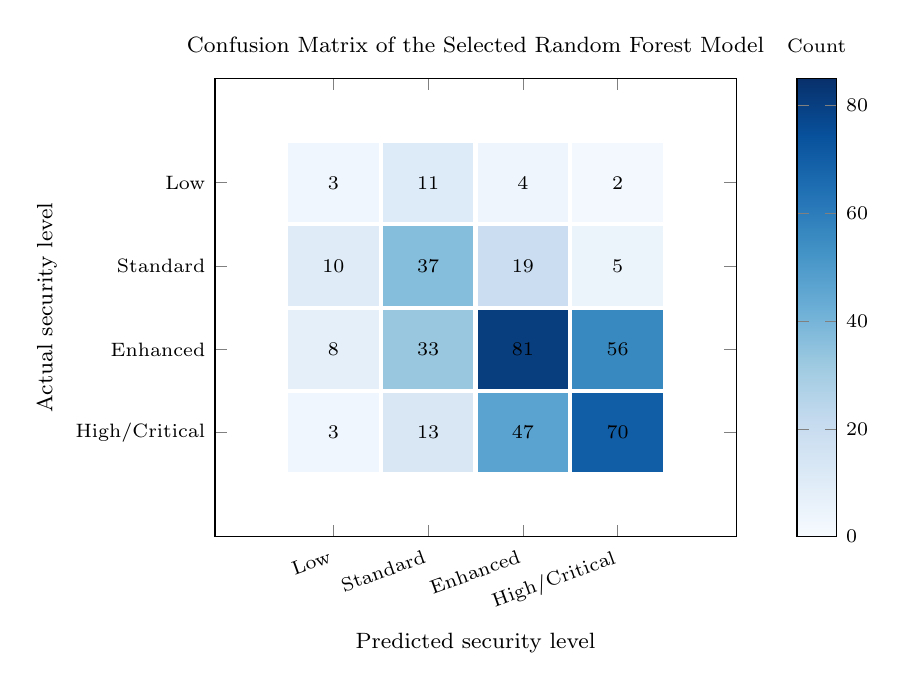
\begin{tikzpicture}
\begin{axis}[
  title={Confusion Matrix of the Selected Random Forest Model},
  title style={font=\footnotesize},
  width=8.2cm, height=7.4cm,
  enlargelimits={abs=0.75}, axis on top,
  colormap/Blues, colorbar,
  colorbar style={title={Count}, title style={font=\scriptsize}, tick label style={font=\scriptsize}},
  point meta min=0, point meta max=85,
  xtick={0,1,2,3}, ytick={0,1,2,3},
  xticklabels={Low,Standard,Enhanced,High/Critical},
  yticklabels={Low,Standard,Enhanced,High/Critical},
  x tick label style={rotate=20, anchor=north east, font=\scriptsize},
  y tick label style={font=\scriptsize},
  xlabel={Predicted security level}, ylabel={Actual security level},
  label style={font=\footnotesize},
  y dir=reverse,
  nodes near coords, nodes near coords style={font=\scriptsize, anchor=center},
]
\addplot[matrix plot*, mesh/cols=4, point meta=explicit, draw=white, line width=1.5pt] table[meta=c] {
x y c
0 0 3
1 0 11
2 0 4
3 0 2
0 1 10
1 1 37
2 1 19
3 1 5
0 2 8
1 2 33
2 2 81
3 2 56
0 3 3
1 3 13
2 3 47
3 3 70
};
\end{axis}
\end{tikzpicture}
\caption{Confusion matrix for the H2 balanced Random Forest survey-target experiment. Values
represent prediction counts.}\label{fig3}
\end{figure}

\begin{table}[h]
\caption{Comparison of Ten-Input and Seven-Input Random Forest Models}\label{tab3}
\begin{tabular}{@{}lcc@{}}
\toprule
Metric & 10-Input RF & 7-Input RF (K7) \\
\midrule
Macro-F1 & 0.389 $\pm$ 0.026 & 0.380 $\pm$ 0.024 \\
Accuracy (\%) & 75.4 $\pm$ 0.8 & 72.5 $\pm$ 1.6 \\
Number of input features & 10 & 7 \\
High/Critical $\rightarrow$ Low/Standard error (\%) & 13.0 & 15.9 \\
\botrule
\end{tabular}
\end{table}

\section{Future Scope of Work}\label{sec9}

In the future, the DEDV system can be improved by using a larger and more diverse dataset to
enhance the classification parameters of the model. Additional data can also help improve the
accuracy of the prediction and improve the identification of the Enhanced class. For practical
applicability the system can be tested in real world scenarios and documents. Furthermore, the
efficiency and execution time of encryption and decryption process can be measured and assessed.
Improvements in decision making process and key management mechanism can be explored to strengthen
the reliability and usability of the proposed system.

\section{Conclusion}\label{sec10}

This paper presents the Dynamic Encryption Digital Vault (DEDV), a framework designed for secure
document storage. The system assigns the document a security level based on contextual attributes
such as sensitivity, usage patterns, access requirements and exposure consequences. The proposed
approach uses Random Forest model to classify the security level and integrate the result with
encryption and key management processes. Random Forest achieved the best macro F1 score of 0.389
for ten-inputs and 0.380 with selected seven-input configuration with fewer input requirements
among the evaluated Machine Learning models. The limited number of records for Enhanced class
affected classification reliability. The system effectiveness will improve with improvements in
data quality and real-world validation. Overall, DEDV provides a unified vault with context aware
document protection through adaptive security level selection.

\bibliography{DEDV_2}

\end{document}
